
\documentclass[master]{thesis-uestc}
\usepackage{listings}  % 引入 listings 宏包,用于显示代码
\title{面向长尾分布数据的自监督预训练故障诊断方法研究}{}

\author{王本浩}{Wang Benhao}
\advisor{周雪\chinesespace 教授}{Dr. Xue Zhou}
\school{电子科技大学(深圳)高等研究院}{Shenzhen Institute for Advanced Study}
\major{电子信息}{Electronic and Information Engineering}
\studentnumber{202222280517}

\begin{document}

\makecover

\begin{chineseabstract}
为了适应日益增长的宽带信号和非线性系统的工程应用,用于分析瞬态电磁散射问题的时域积分方程方法研究日趋活跃。本文以时域积分方程时间步进算法及其快速算法为研究课题,重点研究了时间步进算法的数值实现技术、后时稳定性问题以及两层平面波算法加速计算等,主要研究内容分为四部分。

……

\chinesekeyword{时域电磁散射,时域积分方程,时间步进算法,后时不稳定性,时域平面波算法}
\end{chineseabstract}

\begin{englishabstract}
With the widespread engineering applications ranging from broadband signals and non-linear systems, time-domain integral equations (TDIE) methods for analyzing transient electromagnetic scattering problems are becoming widely used nowadays. TDIE-based marching-on-in-time (MOT) scheme and its fast algorithm are researched in this dissertation, including the numerical techniques of MOT scheme, late-time stability of MOT scheme, and two-level PWTD-enhanced MOT scheme. The contents are divided into four parts shown as follows.

\englishkeyword{Time-domain Electromagnetic Scattering, Time-domain Integral Equation, Marching-on In-time (MOT) Scheme, Late-time Instability, Plane Wave Time-domain (PWTD) Algorithm}
\end{englishabstract}

\thesistableofcontents

\chapter{绪\hspace{6pt}论}

\section{研究工作的背景与意义}
旋转机械作为现代工业中的关键机械设备,长期运行在高温、疲劳、重载的复杂环境中。产生的故障可能会造成严重的事故,造成巨大的经济损失和人员伤亡。智能诊断是预测健康管理(PHM)的关键组成部分,PHM是直升机、航空发动机、风力涡轮机、高速列车等各种旋转机械中最重要的系统之一,旨在有效检测故障。传统的智能诊断方法主要包括使用信号处理方法进行特征提取和使用机器学习方法进行故障分类,这些方法已经取得了相当大的进展。然而,面对异构海量数据,由专家设计和选择的特征提取方法和从信号到条件的映射能力在很大程度上取决于先验知识,既费时又需要经验。因此,如何更精确、更有效地进行诊断仍然是一个具有挑战性的问题。

现实生活中的故障检测数据通常服从长尾分布\citing{nanjing2023faultdetection}长尾分布数据是一种偏态分布,即头部类包含了大部分正常数据,相反地,尾部类包含的故障数据量比较少。用长尾数据训练神经网络时,神经网络的性能易被头部类影响而在尾部类上表现较差,对尾部类样本的错分往往会带来更大的损失,对尾部类样本的研究更具有价值意义。因此如何基于长尾分布的故障检测数据训练故障检测模型是一个具有现实意义的难点问题\citing{cumm2023faultdiagnosis}。目前,在视觉识别长尾学习领域有诸多前沿的长尾学习方法,如变分自编码器\citing{kingma2013auto}、生成对抗网络\citing{goodfellow2020generative}、CB(Class-Balanced) Loss\citing{cui2019class}、自监督学习\citing{yang2020rethinking}、MARC决策面调整算法\citing{wang2023margin},而在故障诊断长尾学习领域常见的方案为半监督学习方法\citing{nanjing2023faultdetection}、集成学习\citing{吴亮2023基于多级学习的长尾分布下交通多目标检测}、样本加权\citing{cumm2023faultdiagnosis},少有前者应用前沿的长尾学习方法在故障诊断长尾学习领域。因此,基于前沿的长尾学习方法提出一个适用于故障诊断领域的长尾学习模型是一个具有现实意义的挑战。

目前,大部分神经网络的训练仍然使用的是有监督范式,需要耗费大量的标注数据,标注这些数据是非常耗时费力的。而自监督的提出就是为了打破对人工标注的依赖,即使在没有标注数据的情况下,也可以高效地训练网络。不同于传统的非监督学习,自监督学习通过人工构造输入数据的代理标签,然后依赖于代理标签设计神经网络的监督训练任务。神经网络从而学习到特征表示。文献\cite{zhang2021federated}指出额外的自监督预训练能够使常规的长尾学习算法获得更高的性能,且验证了自监督预训练在CIFAR-LT、ImageNet-LT等视觉识别长尾数据集上的性能提升。目前,在故障诊断长尾学习领域常见的方案为半监督学习方法、集成学习、样本加权,而少有前者应用前沿自监督预训练方法在故障诊断长尾学习领域。因此,基于自监督预训练的长尾数据故障诊断是一个具有现实意义的挑战。

\section{长尾学习方法的国内外研究历史与现状}
\subsection{长尾学习的发展历程和研究现状}
国内外处理长尾问题通常从三个方面入手。一、样本层面,减少样本数量的欠采样如随机欠采样、NearMiss\citing{shen2016near}、ENN\citing{wilson1972asymptotic};增加样本数量的过采样,如随机过采样、SMOTE\citing{chawla2002smote}、变分自编码器\citing{kingma2013auto}、生成对抗网络\citing{goodfellow2020generative}。二、损失函数层面,使用类平衡的损失函数如以数据频率的逆加权\citing{huang2016learning},OHEM(Online Hard Example Mining),Focal Loss\citing{lin2017focal}以及最新的CB(Class-Balanced) Loss\citing{cui2019class}。三、模型层面,如重复组合少数类样本与抽样的同样数量的多数类样本进行集成学习、半监督和自监督学习\citing{yang2020rethinking}、MARC决策面调整算法\citing{wang2023margin}。

目前,基于长尾分布问题,国内外做出了许多研究。例如:Liu J等人\citing{liu2020deep},介绍了一种基于特征云的数据增强手段,从方差较大的数据分布宽广的头部类中学习到类内多样性并转移到尾部类,并应用于人脸识别。Yang Y等人\citing{yang2020rethinking},介绍了不平衡样本的标签在模型训练中的价值,并提出了用半监督的学习方法使用原模型识别无标签的数据,并以获得伪标签的数据扩充原数据集,同时证明了自监督的模型预训练的有效性,且样本维度越高对性能提升越有效。吴磊等人\citing{wu2023personalized}提出了提出一种面向长尾图像的个性化专家识别算法。该算法在残差网络的基础上构建多专家学习网络,并加入个性化学习模块、信息融合模块与个性化信息增强模块,以两阶段的学习方式提升长尾图像整体的识别准确率与中、尾部类别的识别效果。吴亮等人\citing{吴亮2023基于多级学习的长尾分布下交通多目标检测}构建了多级分组分类器,提升尾部类性能的同时,避免头部类性能损失。然后设计了基于多头注意力机制的分组特征重融合模块,为多级分类器输入更精细的特征。最后,基于多级分类器提出了 Logit 联合调整的方法,以缓解组间的不平衡。Wang Y等人\citing{wang2023margin}介绍了一种对长尾视觉识别学习有效的MARC决策面调整算法,对原模型输出的预测分数额外做一次训练——只用三行代码。Cui Y等人\citing{cui2019class},介绍了CB(Class-Balanced)损失函数,在原损失函数上乘以与“独特”样本数量有关的因子从而缓解类别不平衡。CB因子与超参数β有关,平滑了由1到最常见的不平衡因子1∕n。综上,文献\cite{yang2020rethinking}为自监督预训练模型应用在故障诊断长尾学习领域提供了良好的启示,但半监督学习方法在现实的长尾学习模型可能不适用。文献\cite{wu2023personalized,吴亮2023基于多级学习的长尾分布下交通多目标检测}介绍的集成学习方法削弱样本不平衡效应是常规方法,但单个模型在训练时若融合自监督预训练的方法,性能可能会得到提升。文献\cite{wang2023margin}介绍的决策面调整算法对一般的长尾学习模型都适用,但在故障诊断模型上是否可行有待商榷,且该算法对模型性能提升的理论性解释有待完善。文献\cite{cui2019class}介绍的损失函数有着新颖的思路,但超参数β需要人工选择在应用上可能存在难点。以上大部分为学者在视觉长尾学习领域的研究,此类算法在CIFAR-LT、ImageNet-LT等视觉识别数据集取得了较好的效果,而故障诊断长尾学习领域少有前沿的长尾学习算法的应用。因此,前沿的长尾学习算法在故障诊断长尾学习领域的应用具有很高的研究价值。
\subsection{自监督预训练的发展历程和研究现状}
2019 年 MoCo\citing{He_2020_CVPR} 的横空出世,掀起了视觉自监督学习的热潮。后面 SimCLR\cite{chen2020simple}, BYOL\citing{grill2020bootstrap}, SwAV\citing{caron2020unsupervised} 等主流自监督学习算法相继被提出,自监督学习领域呈现出百花齐放,百家争鸣空前繁荣的景象。2021 年末MAE\citing{he2022masked} 更是将自监督学习带到了一个前所未有的新高度。但是繁荣的背后,自监督学习经历了漫长的迭代和发展过程。

目前,对于自监督预训练,国内外做出了许多研究。例如视觉领域:Yang Y等人\citing{yang2020rethinking},介绍了不平衡样本的标签在模型训练中的价值,并提出了用半监督的学习方法使用原模型识别无标签的数据,并以获得伪标签的数据扩充原数据集,同时证明了自监督预训练的有效性,且样本维度越高对性能提升越有效,为自监督预训练在故障诊断长尾学习领域提供了强力的支撑。Doersch C等人\citing{doersch2015unsupervised} 构建了从一张图片中随机抽取两个块,然后让模型来预测一个块相对于另外一个块的位置的自监督预训练任务。Zhang R等人\citing{zhang2016colorful}构建了涂色的自监督预训练任务,将图片转换到 CIE Lab 颜色空间,然后将 L 通道喂入模型,然后让模型去预测 a, b 通道的数值。Gidaris S等人\citing{gidaris2018unsupervised}人为地将图像旋转不同角度,并将旋转角度作为有监督模型训练的代理标签。实验结果表明,该模型可以通过预测旋转角度来学习图像的语义特征,从而为后续任务提供有效的特征表示。无独有偶,近些年在故障诊断领域,自监督预训练的研究也得到了学者们的关注。例如:Zhang T等人\citing{zhang2022prior}建立了以先验知识为代理标签的自监督预训练任务训练卷积自编码器模型,并在小样本学习上得到了应用。Senanayaka等人\citing{senanayaka2020toward}以One-Class SVM输出的标签作为代理标签,使用自监督预训练的卷积神经网络做故障特征提取。W. Zhang等人\citing{zhang2021federated}将时域信号划分为块,通过交换信号块的位置人为制造“伪数据”,自监督预训练的训练目标为区分数据是否为“伪数据”。自监督预训练在视觉学习领域的研究百花齐放,故障诊断领域的研究也蒸蒸日上。综上,文献\cite{doersch2015unsupervised,zhang2016colorful,gidaris2018unsupervised}为视觉领域的自监督预训练方法,应用在故障诊断模型存在困难,但为故障诊断模型的自监督预训练设计提供了思想上的启示。如文献\cite{senanayaka2020toward}的One-Class SVM构造标签在多分类目标上使用聚类算法可能会更有通用性。文献\cite{zhang2021federated}所提的交换信号块的位置预测样本真伪可能与文献\cite{doersch2015unsupervised}的预测图片块的位置可以结合。而文献\cite{zhang2022prior,senanayaka2020toward,zhang2021federated}故障诊断领域的自监督预训练在学习任务上有很大的创新空间,且在长尾学习领域的应用稍有欠缺。因此,故障诊断领域的自监督预训练还处于萌芽阶段,参考视觉领域的前沿自监督学习任务在现有故障诊断领域的自监督预训练方法的基础上提出更具创新性和更高性能的自监督预训练任务是有研究价值和意义的挑战。

\section{本文的主要贡献与创新}
本论文以时域积分方程时间步进算法的数值实现技术、后时稳定性问题以及两层平面波加速算法为重点研究内容,主要创新点与贡献如下:

\section{本论文的结构安排}
本文的章节结构安排如下:

\chapter{长尾学习理论基础与轴承故障数据集}
\section{长尾学习相关理论}
不平衡数据在现实世界中无处不在,大规模数据集通常表现为长尾分布。长尾分布的学习亦是故障诊断领域中常见挑战,例如正常工作状态多,故障工作状态少,或是常见故障状态和罕见故障状态的样本个数差异。现实生活中的故障检测数据通常服从长尾分布,长尾分布数据是一种偏态分布,如图\ref{fig_long_tail}所示,在现实生活中,大规模的训练样本呈现典型的长尾分布,即头部类别的样本个数较多,而尾部类别的样本个数较少,样本个数逐渐降低的分布。用长尾数据训练神经网络时,神经网络的性能易被头部类影响而在尾部类上表现较差,对尾部类样本的错分往往会带来更大的损失,对尾部类样本的研究更具有价值意义。因此如何基于长尾分布的故障检测数据训练故障检测模型是一个具有现实意义的难点问题。
\begin{figure}[h]
    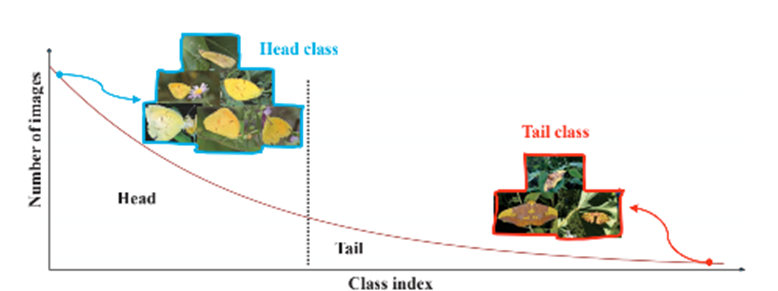
\includegraphics[width=10cm]{long_tail.png}
    \caption{长尾分布示意图}
    \label{fig_long_tail}
\end{figure}

长尾分布的样本具有非常显著的样本不均衡问题,导致训练好的模型易偏向于头部类,从而损害了对尾部类的识别效果。如图\ref{tsne_mean_distribution}所示,样本个数均衡时,各个类别之间具有清晰的区分边界,各类都占据了宽广的特征空间。而当某些类的样本个数减少呈现样本分布失衡的长尾分布时,如图\ref{tsne_lt_distribution}所示,尾部类在特征空间的分布十分狭窄,并依附在头部类附近,从而扭曲了特征空间,损害了类间的多样性和区分性。
这对现代深度学习框架提出了一个重大挑战,即使使用数据重采样方法或类平衡损失等专门技术,在极端类不平衡的情况下,仍然会出现显著的性能下降。因此,为了进一步应对这一挑战,了解类不平衡学习所带来的不同特征至关重要。然而,与平衡数据不同的是,不平衡学习背景下的标签扮演着令人惊讶的有争议的角色,这导致了标签价值的持续困境:一方面,有标签监督的学习算法通常比无监督的学习算法产生更准确的分类器,这表明了标签的积极价值;然而,另一方面,不平衡的标签在学习过程中自然会产生“标签偏差”,其中大多数类别可以显著地驱动决策边界,表明标签的负面影响。因此,不平衡的标签似乎是一把双刃剑。
\begin{figure}[h]
    \subfloat[]{
        \label{tsne_mean_distribution}
        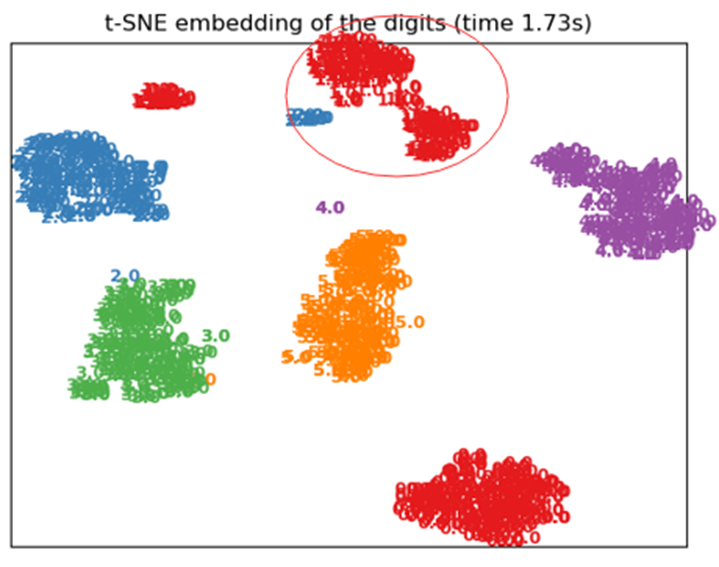
\includegraphics[width=6.77cm]{tsne_mean_distribution.png}
    }
    \subfloat[]{
        \label{tsne_lt_distribution}
        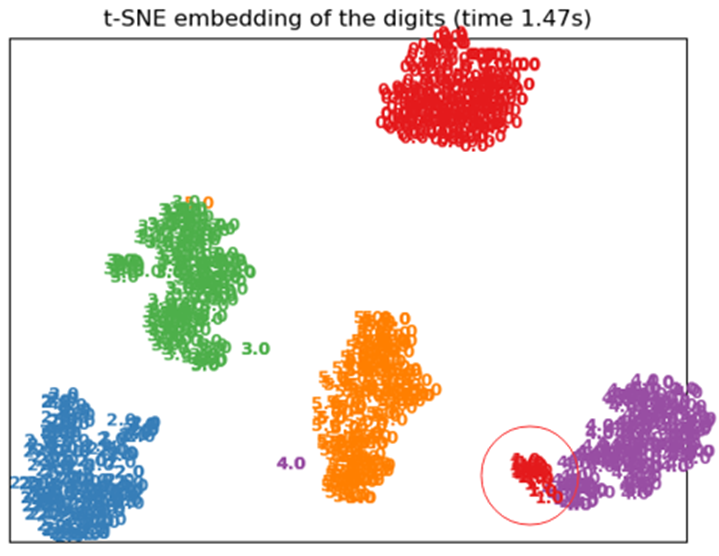
\includegraphics[width=6.77cm]{tsne_lt_distribution.png}
    }
    \caption{均匀/长尾分布数据的tsne图(a)样本均匀分布时的T-SNE分布图;(b)尾部类“1”类样本个为30,头部类样本个数为180个时的T-SNE分布图}
    \label{long-tail result}
\end{figure}

\section{自监督学习相关理论}
自监督学习是一种范式,利用“代理任务”(pretext)从大规模的无标签数据本身的内在结构挖掘通用的表征信息,通过这种构造的监督信息对网络进行训练,从而可以学习到对下游任务有价值的表征。如图(todo:补充SSL流程框图)所示,自监督学习分为两个阶段:(1)自监督预训练阶段。完全放弃标签信息,专注于数据本身,通过自监督学习进行预训练。从不平衡数据中学习标签不可知的特征表示,减少类别偏差对初始化的影响。(2)微调阶段。使用第一阶段中通过自监督预训练的网络权重作为初始化。在此基础上,可以使用任何标准的不平衡学习技术进行进一步训练,学习最终的分类模型。由于预训练阶段和正常训练阶段是独立的,自监督学习可以与现有的不平衡学习方法无缝结合,增强模型性能,且自监督预训练阶段不依赖标签,使得网络能学习到更通用、更鲁棒的特征表示,从而避免了类别不平衡对特征学习的负面影响。

(todo: 1.补充公式理论Rethinking the Value of Labels for Improving Class-Imbalanced Learning2.补充SSL流程框图)
\section{孪生网络与对比学习相关理论}
对比学习是一种学习方法,侧重于通过对比正反两方面的实例来提取有意义的表征。它利用的假设是,在学习到的嵌入空间中,相似的实例应靠得更近,而不相似的实例应离得更远。通过将学习作为一项辨别任务,对比学习允许模型捕捉数据中的相关特征和相似性。对比学习主要分为监督对比学习和自监督对比学习两大类。

监督对比学习是对比学习的一个分支,它利用标记数据来明确训练模型以区分相似和不相似的实例。在监督对比学习中,模型在数据点对及其标签上进行训练,指示数据点是否相似或不相似。目标是学习一个表示空间,其中相似的实例聚集得更近,而不同的实例则被推开。一种流行的方法是信息噪声对比估计(InfoNCE)损失函数。 InfoNCE损失在学习的表示空间中最大化正样本之间的一致性并最小化负样本之间的一致性。通过优化此目标,模型学会区分相似和不相似的实例,从而提高下游任务的性能。

自监督对比学习采用不同的方法,从未标记的数据中学习表示,而不依赖于显式标签。 自监督对比学习利用借口任务的设计,从未标记的数据创建正负对。这些借口任务经过精心设计,旨在鼓励模型捕获数据中有意义的特征和相似性。自监督对比学习中常用的借口任务之一是生成增强视图。这涉及创建同一实例的多个增强版本并将它们视为正对,而来自不同样本的实例则被视为负对。通过训练模型来区分这些对,它可以学习捕获更高级别的语义信息并很好地推广到下游任务。
(todo:补充监督对比学习和自监督对比学习框图)
\section{相关数据集介绍}
\subsection{CWRU数据集介绍}

\chapter{基于孪生网络对比学习的自监督预训练方法研究}
\section{引言}
\section{模型整体架构及其模块设计}
\subsection{简单暹罗孪生网络}
\begin{figure}[h]
    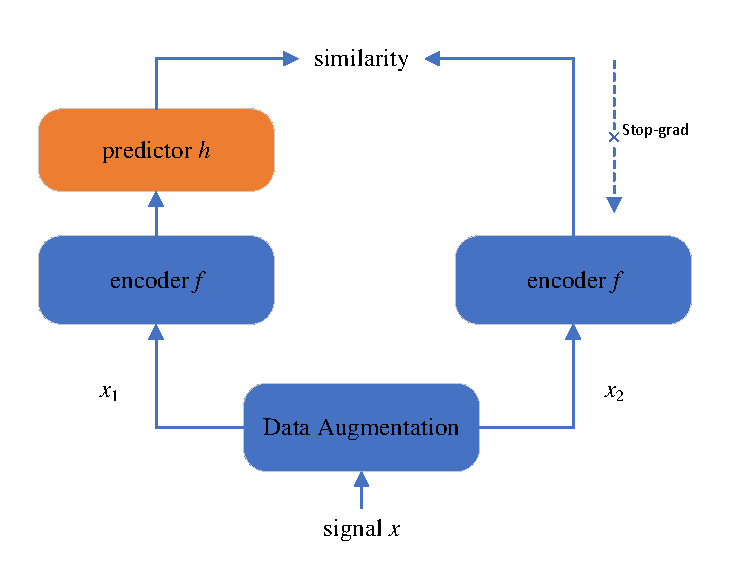
\includegraphics[width=12cm]{simsiam_arch.pdf}
    \caption{简单暹罗孪生网络}
    \label{simsiam_arch}
\end{figure}
简单暹罗孪生网络(SimSiam——Simple Siamese)\citing{chen2021exploring}架构(图\ref{simsiam_arch})将信号$x$中的两个随机增强视图$x_1$和$x_2$作为输入。这两个视图由编码器网络$f$处理,该网络由骨干网络(例如ResNet\citing{he2016deep})和投影MLP头部组成。编码器$f$在两个视图之间共享权重。预测MLP头部$h$转换一个视图的输出并将其与另一个视图进行匹配。将两个输出向量表示为$p_1 \triangleq h(f(x_1))$和$p_2 \triangleq f(x_2)$,我们最小化它们的负余弦相似度:
\begin{equation}
    \mathcal{D}(p_1, z_2) = -\frac{p_1}{\|p_1\|_2} \cdot \frac{z_2}{\|z_2\|_2}
    \label{eq:distance}
\end{equation}  
其中,$\|\cdot\|_2$ 是 $\ell_2$范数。定义对称损失函数
\begin{equation}
    \mathcal{L} = \frac{1}{2} \mathcal{D}(p_{1}, z_{2}) + \frac{1}{2} \mathcal{D}(p_{2}, z_{1})
\label{eq:cos_loss}
\end{equation}
该损失函数作用于单段信号,总损失值在计算所有信号的损失后取平均值。损失函数的最小值为-1。

方法中一个重要的组件是梯度停止(stop-grad)操作(图 1)。我们通过修改公式(\ref{eq:distance}) 来实现它:
\begin{equation}
    D(p_1, \text{stopgrad}(z_2))
\label{eq:stopgrad}
\end{equation}
这意味着在这一项中,\( z_2 \) 被视为常数。类似地,公式(\ref{eq:cos_loss}) 的实现形式为:
\begin{equation}
\mathcal{L} = \frac{1}{2} D(p_1, \text{stopgrad}(z_2)) + \frac{1}{2} D(p_2, \text{stopgrad}(z_1))
\label{eq:cos_loss_stopgrad}
\end{equation}
第一项中 \( x_2 \) 的编码器不会从 \( z_2 \) 接收梯度,但在第二项中会从 \( p_2 \) 接收梯度(反之亦然,对于 \( x_1 \) 也是如此)。即在这一项中,\( z_2 \) 被视为常数。

简单暹罗孪生网络的伪代码如表\ref{table:simsiam_code}所示。

\begin{table}
    \caption{简单暹罗孪生网络的伪代码,用Pytorch描述}
    \begin{tabular}{@{}l@{}} % 使用 @{} 去掉默认的左右边距,l 表示左对齐
    \toprule
    \multicolumn{1}{@{}l@{}}{\textbf{简单暹罗孪生网络Pytorch伪代码}} \\ % 左对齐文本
    \midrule
    \begin{lstlisting}[basicstyle=\ttfamily,frame=none]
#f: 骨干网络 + 投影 MLP
#h: 预测 MLP
for x in loader:  # 加载一个包含 n 个样本的小批量数据 x
    x1, x2 = aug(x), aug(x)  # 随机数据增强
    z1, z2 = f(x1), f(x2)  # 投影,形状为 n-by-d
    p1, p2 = h(z1), h(z2)  # 预测,形状为 n-by-d
    L = D(p1, z2)/2 + D(p2, z1)/2  # 损失函数

    L.backward()  # 反向传播
    update(f, h)  # SGD 更新

def D(p, z):  # 负余弦相似度
    z = z.detach()  # 停止梯度
    p = normalize(p, dim=1)  # 对 p 进行 L2 归一化
    z = normalize(z, dim=1)  # 对 z 进行 L2 归一化
    return -(p * z).sum(dim=1).mean()  # 计算负余弦相似度
    \end{lstlisting} \\
    \bottomrule
    \end{tabular}
    \label{table:simsiam_code}
\end{table}
\subsection{简单暹罗孪生故障诊断网络}
\begin{figure}[h]
    \centering
    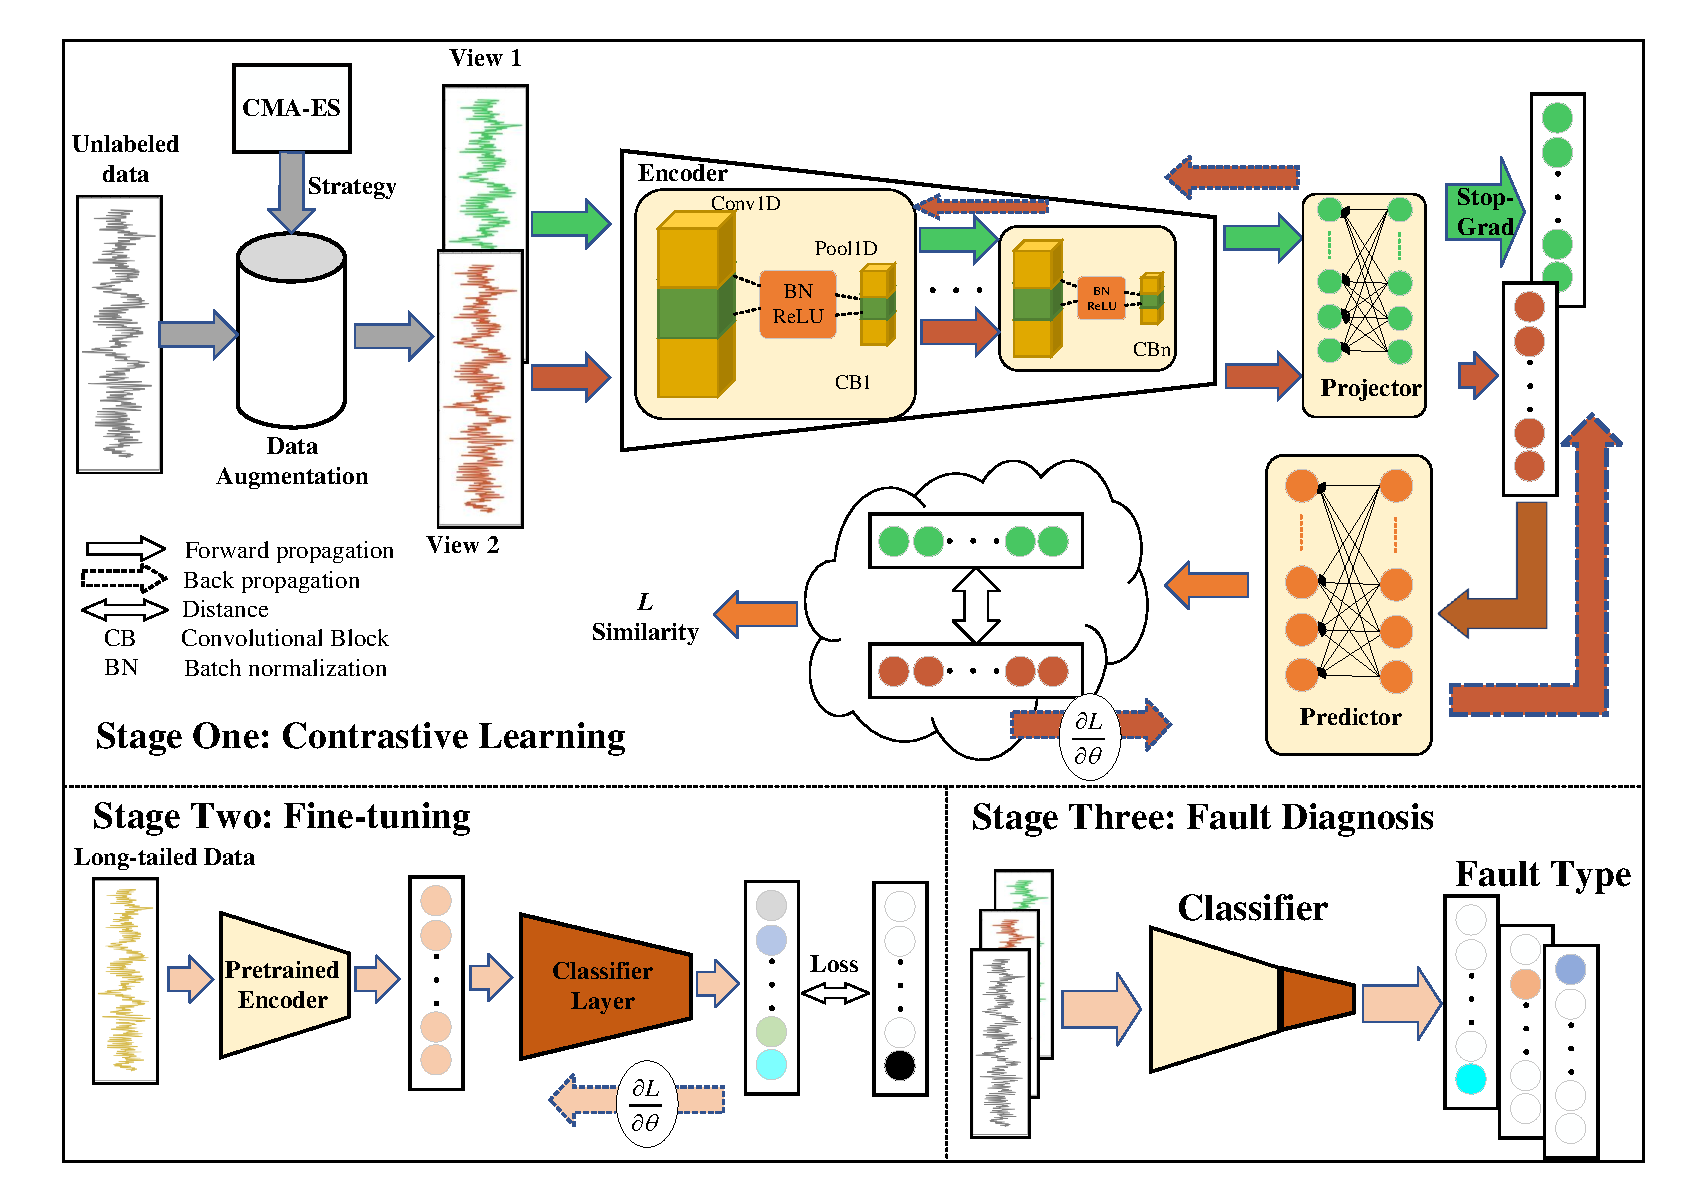
\includegraphics[width=16cm]{simsiam_net.pdf}
    \caption{简单暹罗孪生故障诊断网络}
    \label{simsiam_net}
\end{figure}
提出的用于故障诊断的简单暹罗孪生网络如图\ref{simsiam_net}所示,以下是架构的介绍。

1)\textbf{数据增强(Data Augmentations)}:
在对比表示学习算法中,数据增强(DA)起着至关重要的作用。成功地从振动信号中提取可区分的故障特征,依赖于为同一样本生成不同视图的质量。我们知道,面向图像的最新(SOTA)对比表示学习算法广泛使用多种数据增强方法,而针对序列数据的增强方法则相对较少。
此外,用于对比学习生成正样本对的增强方法必须满足一个条件,即加入样本的噪声不能改变其语义含义。因此,我们选择了以下九种数据增强方法:

\begin{itemize}
    \item \textbf{掩码(Random Masked)}:用于遮盖输入数据的一部分,即随机挑选信号的某些部分用 0 替代,通常是在序列数据或图像数据中随机选择部分区域进行掩码处理。这有助于模型在训练时学会忽略一些无关信息,从而提高其鲁棒性。

    \item \textbf{添加高斯噪声(Adding Gaussian Noise)}:将高斯噪声添加到数据中的方法,常用于增强模型的鲁棒性。通过这种方式,模型在训练过程中能够适应噪声,并提升其在实际应用中的性能,尤其是在存在噪声的环境中。

    \item \textbf{相位扰动(Phase Perturbation)}:修改信号的频率域中的相位信息,而保持幅度不变来生成新的数据样本。这种方法保留了信号的整体结构,但引入了细微的扰动,用于提高模型的泛化能力。

    \item \textbf{块打乱(RandomChunkShuffle)}:将时间序列数据分割成多个块,然后随机打乱这些块的顺序。这样可以创建不同的序列变体,增加模型对数据变异的适应能力,同时保持整体的语义不变。

    \item \textbf{随机缩放(Random Scaled)}:对数据进行随机幅度缩放来增强数据的方法。通过改变数据的尺度,模型能够学习到不同幅度下的数据模式,从而提升其泛化能力。

    \item \textbf{随机绝对值(Random Abs)}:对数据应用绝对值操作,将负值转换为正值或去掉负号。这个方法帮助模型处理包含负值的情形,增强其鲁棒性。

    \item \textbf{竖直翻转(Random Vertical Flip)}:随机地将数据进行竖直翻转来创建新的样本。这对于一些对竖直方向变化不敏感的任务非常有效。

    \item \textbf{水平翻转(Random Horizontal Flip)}:随机将图像或数据进行水平翻转,生成新的样本。这种方法对于对称性较强的数据非常有效,能增强模型的鲁棒性。

    \item \textbf{时移(Time Shift)}:将数据在时间轴上平移一定的时间步长来生成新的样本。这种方法可以帮助模型学会适应时间序列数据中事件的变化位置,提升其对时间依赖的理解能力。
\end{itemize}

同一输入信号分别经过上述数据增强方法后的视图如图\ref{data_augmentation}所示。
\begin{figure}[h]
    \centering
    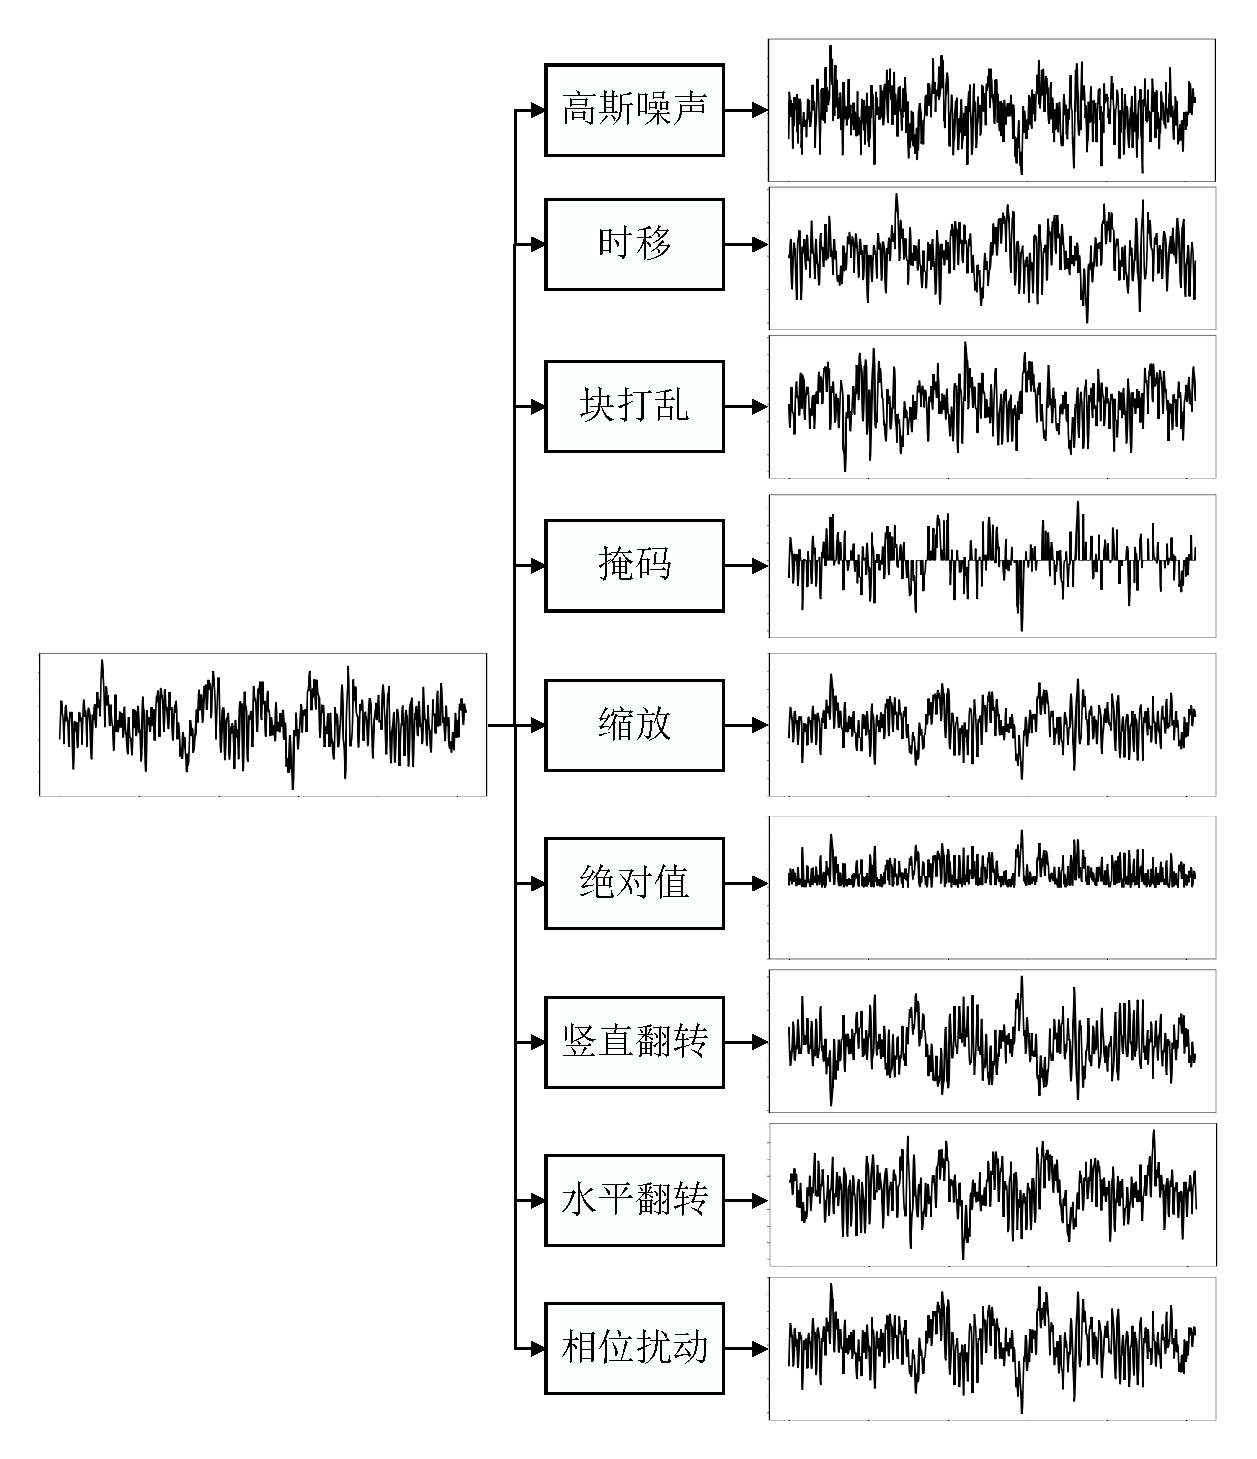
\includegraphics[width=10cm]{data_augmentation.pdf}
    \caption{数据增强示意图}
    \label{data_augmentation}
\end{figure}

2)\textbf{编码器(Encoder),预测器(Predictor)和分类器(Classifier)}:编码器是该算法中故障诊断的关键部分。我们主要使用其潜在编码来完成分类任务。由于简单暹罗网络是一个框架,我们可以根据需要构建编码器模型和预测器,其中预测器是一个相对简单的非线性函数。在第二阶段,需要在预训练的编码器后添加一个分类器层用于故障诊断,如图\ref{simsiam_net}所示。为了方便起见,我们使用多个常规的卷积神经网络(CNN)块来构建编码器,并使用全连接层来构建预测器和分类器。每个卷积块(CB)包括四个层:一个 1-D 卷积层\( f_{\text{BN}} \)、一个激活函数层 \( f_{\text{ReLU}} \),以及一个池化层 \( f_{\text{Pool}} \)。 方程(\ref{eq:CNN})展示了 1-D 卷积层的操作,其中输入的形状为 \( (N, C_{\text{in}}, L) \),输出的形状为 \( (N, C_{\text{out}}, L_{\text{out}}) \),其中 \( N \) 是样本的数量,\( C \) 表示通道数,\( L \) 表示数据的长度。
\begin{equation}
    \begin{aligned}
    \operatorname{out}(N_i, C_{\mathrm{out}_j}) &= \operatorname{bias}(C_{\mathrm{out}_j}) + \sum_{k=0}^{C_{\mathrm{in}}-1} \operatorname{weight}(C_{\mathrm{out}_j}, k) \otimes \operatorname{input}(N_i, k).
    \end{aligned}
    \label{eq:CNN}
    \end{equation}
BN 层 \( f_{\text{BN}} \) 用于加速训练过程并减少由于层输入分布不同而导致的内部协变量偏移(ICS)的影响 \citing{ioffe2015batch},当模型较深时,这种影响尤为严重。公式(\ref{eq:BN})展示了批归一化的过程。
\begin{equation}
    f_{\text{BN}}(x_i, \mathbf{x}) = \gamma \frac{x_i - \mathbb{E}(\mathbf{x})}{\sqrt{\sigma(\mathbf{x})^2 + \epsilon}} + \beta
\label{eq:BN}
\end{equation}    
\begin{equation}
\mathbb{E}(\mathbf{x}) = \frac{1}{N}\sum_{i=1}^N x_i
\label{eq:exp_BN}
\end{equation}
\begin{equation}
\sigma(\mathbf{x}) = \sqrt{\frac{1}{N}\sum_{i=1}^N (x_i - \mathbb{E}(\mathbf{x}))^2}
\label{eq:sigma_BN}
\end{equation}
其中 \( x \) 是整个小批量(mini batch)的向量,批量大小为 \( N \),\( x_i \) 表示小批量中的第 \( i \) 个样本。  
\( \mathbb{E}(x) \) 和 \( \sigma(x) \) 分别表示向量批量的均值和方差,如公式 (\ref{eq:exp_BN}) 和 (\ref{eq:sigma_BN}) 所示。\( \epsilon \) 是一个超参数,通常设置为 \( 10^{-5} \),而 \( \gamma \) 和 \( \beta \) 分别是缩放因子和偏移因子,它们是可学习的参数,初始值分别设置为 1 和 0。

激活层 \( f_{\text{ReLU}} \) 可以表示为公式 (\ref{eq:relu}):
\begin{equation}
    f_{\text{ReLU}} = \max(0, x)
    \label{eq:relu}
\end{equation}

\( x_i^{(n)} \) 表示通过第 \( n \) 个卷积块(CB)的第 \( i \) 个输出向量,可以用公式 (\ref{eq:output_of_encoder}) 表示:
\begin{equation}
    \begin{aligned}
    x_i^{(n)} = f_{\text{Pool}}\bigl\{f_{\text{ReLU}}\bigl[f_{BN}\Bigl(f_{\text{conv}}\bigl(\mathbf{x}^{(n-1)}\bigr), f_{\text{conv}}\Bigl(x_i^{(n-1)}\Bigr)\Bigr)\bigr]\bigr\}
    \end{aligned}
    \label{eq:output_of_encoder}
\end{equation}

3)\textbf{优化器(Optimizer)}:模型的训练不需要使用大批量优化器,例如分层自适应速率缩放(LARS)\citing{you2017large},因为所提出的方法可以在典型批量大小下工作,而不依赖于大批量训练。我们使用 SGD 优化器训练模型。网络参数通过公式 (\ref{eq:SGD}) 更新。
\begin{equation}
    \theta_{l+1} = \theta_l - \eta_l \cdot \nabla_{\theta} \mathcal{L}(\mathbf{x}; \theta_l)
\label{eq:SGD}
\end{equation}
其中 \( \theta_t \) 表示时间 \( t \) 时的可学习参数,\( \eta_t \) 表示时间 \( t \) 时的学习率,\( L(\cdot) \) 表示损失函数。

4)\textbf{微调(Fine-tuning)}:在对比学习阶段完成后,我们从模型中取出训练好的编码器 \( f \),并将其与一个多层感知器(MLP)模块连接,我们用带标签的数据微调构建一个完整的分类器用于故障诊断任务,从而使模型获得分类能力。以准确率为性能指标,如公式(\ref{eq:acc}):
\begin{equation}
    \text{Accuracy} = \frac{TN + TP}{TN + TP + FP + FN}
    \label{eq:acc}
\end{equation}
其中,\( TN \) 表示真阴性,即被正确预测为阴性的阴性样本数量。真阳性(\( TP \))表示被模型正确判断为阳性的阳性样本数量。假阳性(\( FP \))表示被错误分类为阴性的阳性样本数量。假阴性(\( FN \))表示被错误分类为阳性的阴性样本数量。

5)\textbf{故障诊断(Fault Diagnosis)}:在完成微调后,即可将模型应用于真实输入信号的故障诊断,以预测故障类别。
\begin{figure}[h]
    \centering
    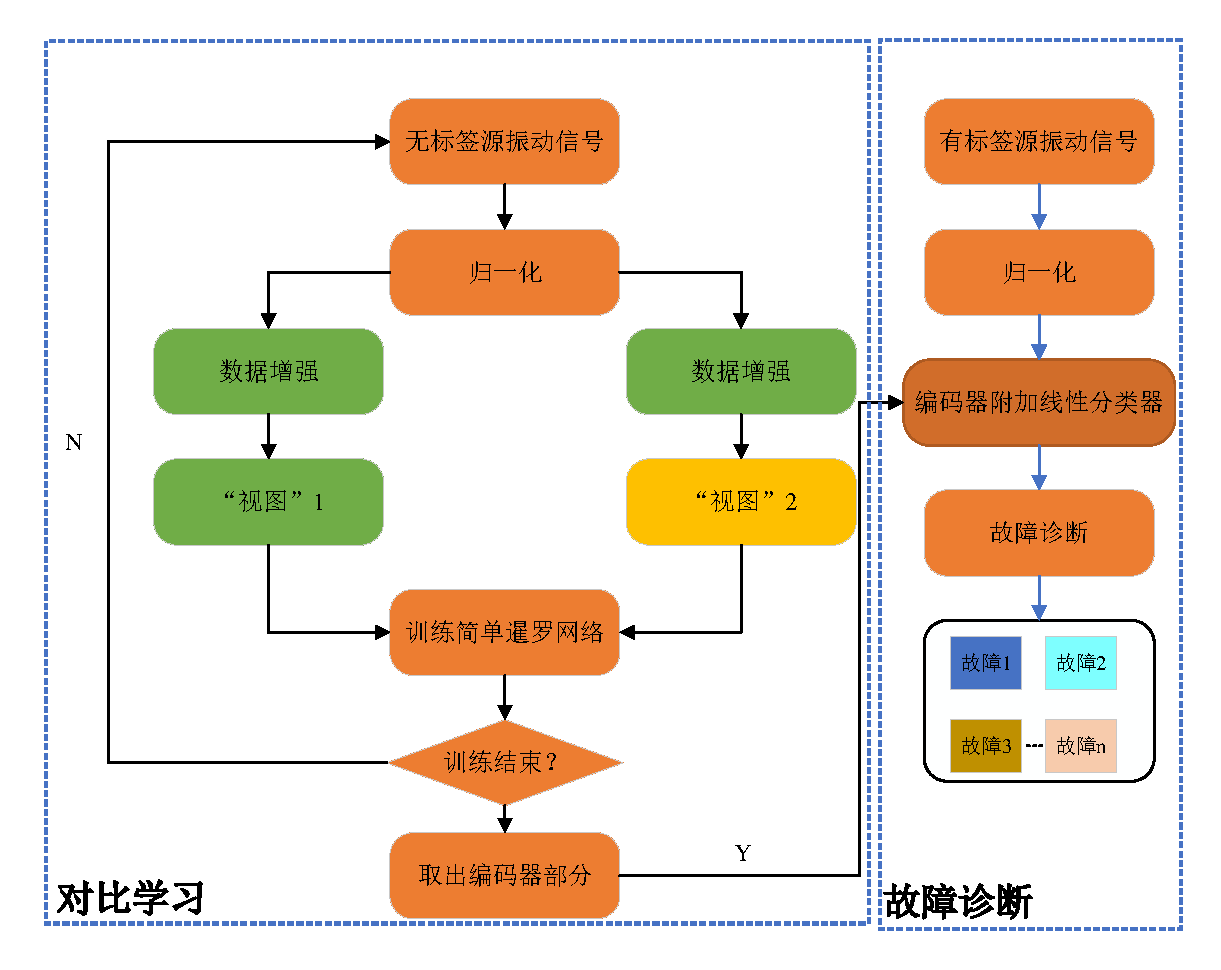
\includegraphics[width=14cm]{simsiam_fault_diag_procedure.pdf}
    \caption{简单暹罗孪生故障诊断网络的训练流程图}
    \label{simsiam_fault_diag_procedure}
\end{figure}
简单暹罗孪生故障诊断网络的训练过程如图\ref{simsiam_fault_diag_procedure}所示。首先,我们需要对所有未标记的振动样本进行归一化预处理,并使用数据增强方法生成输入样本的两个不同视图作为正样本对。我们将正样本对输入模型,然后按照算法表\ref{table:simsiam_code}所示的流程训练模型。训练过程完成后,我们取出编码器,在其最后一层后附加一个线性分类层,并使用标记样本对模型进行微调。线性分类层也可以用其他分类器(如 K 近邻(KNN)和支持向量机(SVM))替换。

\subsection{基于CMA-ES优化器的最优数据增强策略搜索算法}
简单暹罗孪生网络的一个难以接受的平凡解是所有输出都“坍塌”为一个常数。简单暹罗孪生网络利用数据增强生成两个视图,并直接最大化同一输入的两个视图的相似性,即不使用负样本对。因此简单暹罗孪生网络极大程度上依赖于数据增强的效果,而人工筛选数据增强十分耗时耗力且难以获得最优解。该节提出了基于CMA-ES优化器的最优数据增强策略搜索算法,CMA-ES(Covariance Matrix Adaptation Evolution Strategy,协方差矩阵自适应进化策略)是一种用于连续优化问题的进化算法。它是一种基于种群的优化方法,通过自适应调整协方差矩阵来指导搜索方向,从而在高维空间中高效地找到全局最优解。CMA-ES 在解决非线性、非凸、高维优化问题时表现出色,广泛应用于机器学习、工程优化和科学研究中。CMA-ES 的更新规则如下:

1. 采样新解:
\begin{equation}
\mathbf{x}_k^{(g+1)} = \mathbf{m}^{(g)} + \sigma^{(g)} \cdot \mathcal{N}(0, \mathbf{C}^{(g)})
\label{eq:sample}
\end{equation}
其中:
\begin{itemize}
    \item \(\mathbf{x}_k^{(g+1)}\) 是第 \(g+1\) 代中的第 \(k\) 个候选解,
    \item \(\mathbf{m}^{(g)}\) 是第 \(g\) 代的均值向量,
    \item \(\sigma^{(g)}\) 是第 \(g\) 代的步长,
    \item \(\mathbf{C}^{(g)}\) 是第 \(g\) 代的协方差矩阵,
    \item \(\mathcal{N}(0, \mathbf{C}^{(g)})\) 是从多元正态分布中采样的随机向量。
\end{itemize}

2. 更新均值:
\begin{equation}
\mathbf{m}^{(g+1)} = \sum_{i=1}^{\mu} w_i \mathbf{x}_{i:\lambda}^{(g+1)}
\label{eq:mean_update}
\end{equation}
其中:
\begin{itemize}
    \item \(\mu\) 是选择的父代数量,
    \item \(w_i\) 是权重系数,
    \item \(\mathbf{x}_{i:\lambda}^{(g+1)}\) 是第 \(g+1\) 代中适应度排名前 \(\mu\) 的候选解。
\end{itemize}

3. 更新协方差矩阵:
\begin{equation}
\mathbf{C}^{(g+1)} = (1 - c_1 - c_\mu) \mathbf{C}^{(g)} + c_1 \mathbf{p}_c^{(g+1)} (\mathbf{p}_c^{(g+1)})^\top + c_\mu \sum_{i=1}^{\mu} w_i \mathbf{y}_{i:\lambda}^{(g+1)} (\mathbf{y}_{i:\lambda}^{(g+1)})^\top
\label{eq:covariance_update}
\end{equation}
其中:
\begin{itemize}
    \item \(c_1\) 和 \(c_\mu\) 是学习率,
    \item \(\mathbf{p}_c^{(g+1)}\) 是进化路径,
    \item \(\mathbf{y}_{i:\lambda}^{(g+1)} = (\mathbf{x}_{i:\lambda}^{(g+1)} - \mathbf{m}^{(g)}) / \sigma^{(g)}\)。
\end{itemize}

4. 更新步长:
\begin{equation}
\sigma^{(g+1)} = \sigma^{(g)} \exp\left(\frac{c_\sigma}{d_\sigma} \left(\frac{\|\mathbf{p}_\sigma^{(g+1)}\|}{\mathbb{E}[\|\mathcal{N}(0, \mathbf{I})\|]} - 1\right)\right)
\label{eq:stepsize_update}
\end{equation}
其中:
\begin{itemize}
    \item \(c_\sigma\) 是步长学习率,
    \item \(d_\sigma\) 是阻尼系数,
    \item \(\mathbf{p}_\sigma^{(g+1)}\) 是步长进化路径,
    \item \(\mathbb{E}[\|\mathcal{N}(0, \mathbf{I})\|]\) 是标准正态分布向量的期望范数。
\end{itemize}

我们将寻找最佳数据增强策略的问题形式化为一个搜索问题(见图 \ref{CMA-ES})。我们的方法由两个组件组成:搜索算法和搜索空间。在高层次上,搜索算法(实现为CMA-ES)采样一个数据增强策略 \( S \),该策略包含有关使用哪种图像处理操作、每批次中使用该操作的概率以及操作幅度的信息。我们方法的关键在于,策略 \( S \) 将用于训练具有固定架构的神经网络,其验证准确率 \( R \) 将返回以评估适应度。
\begin{figure}[h]
    \centering
    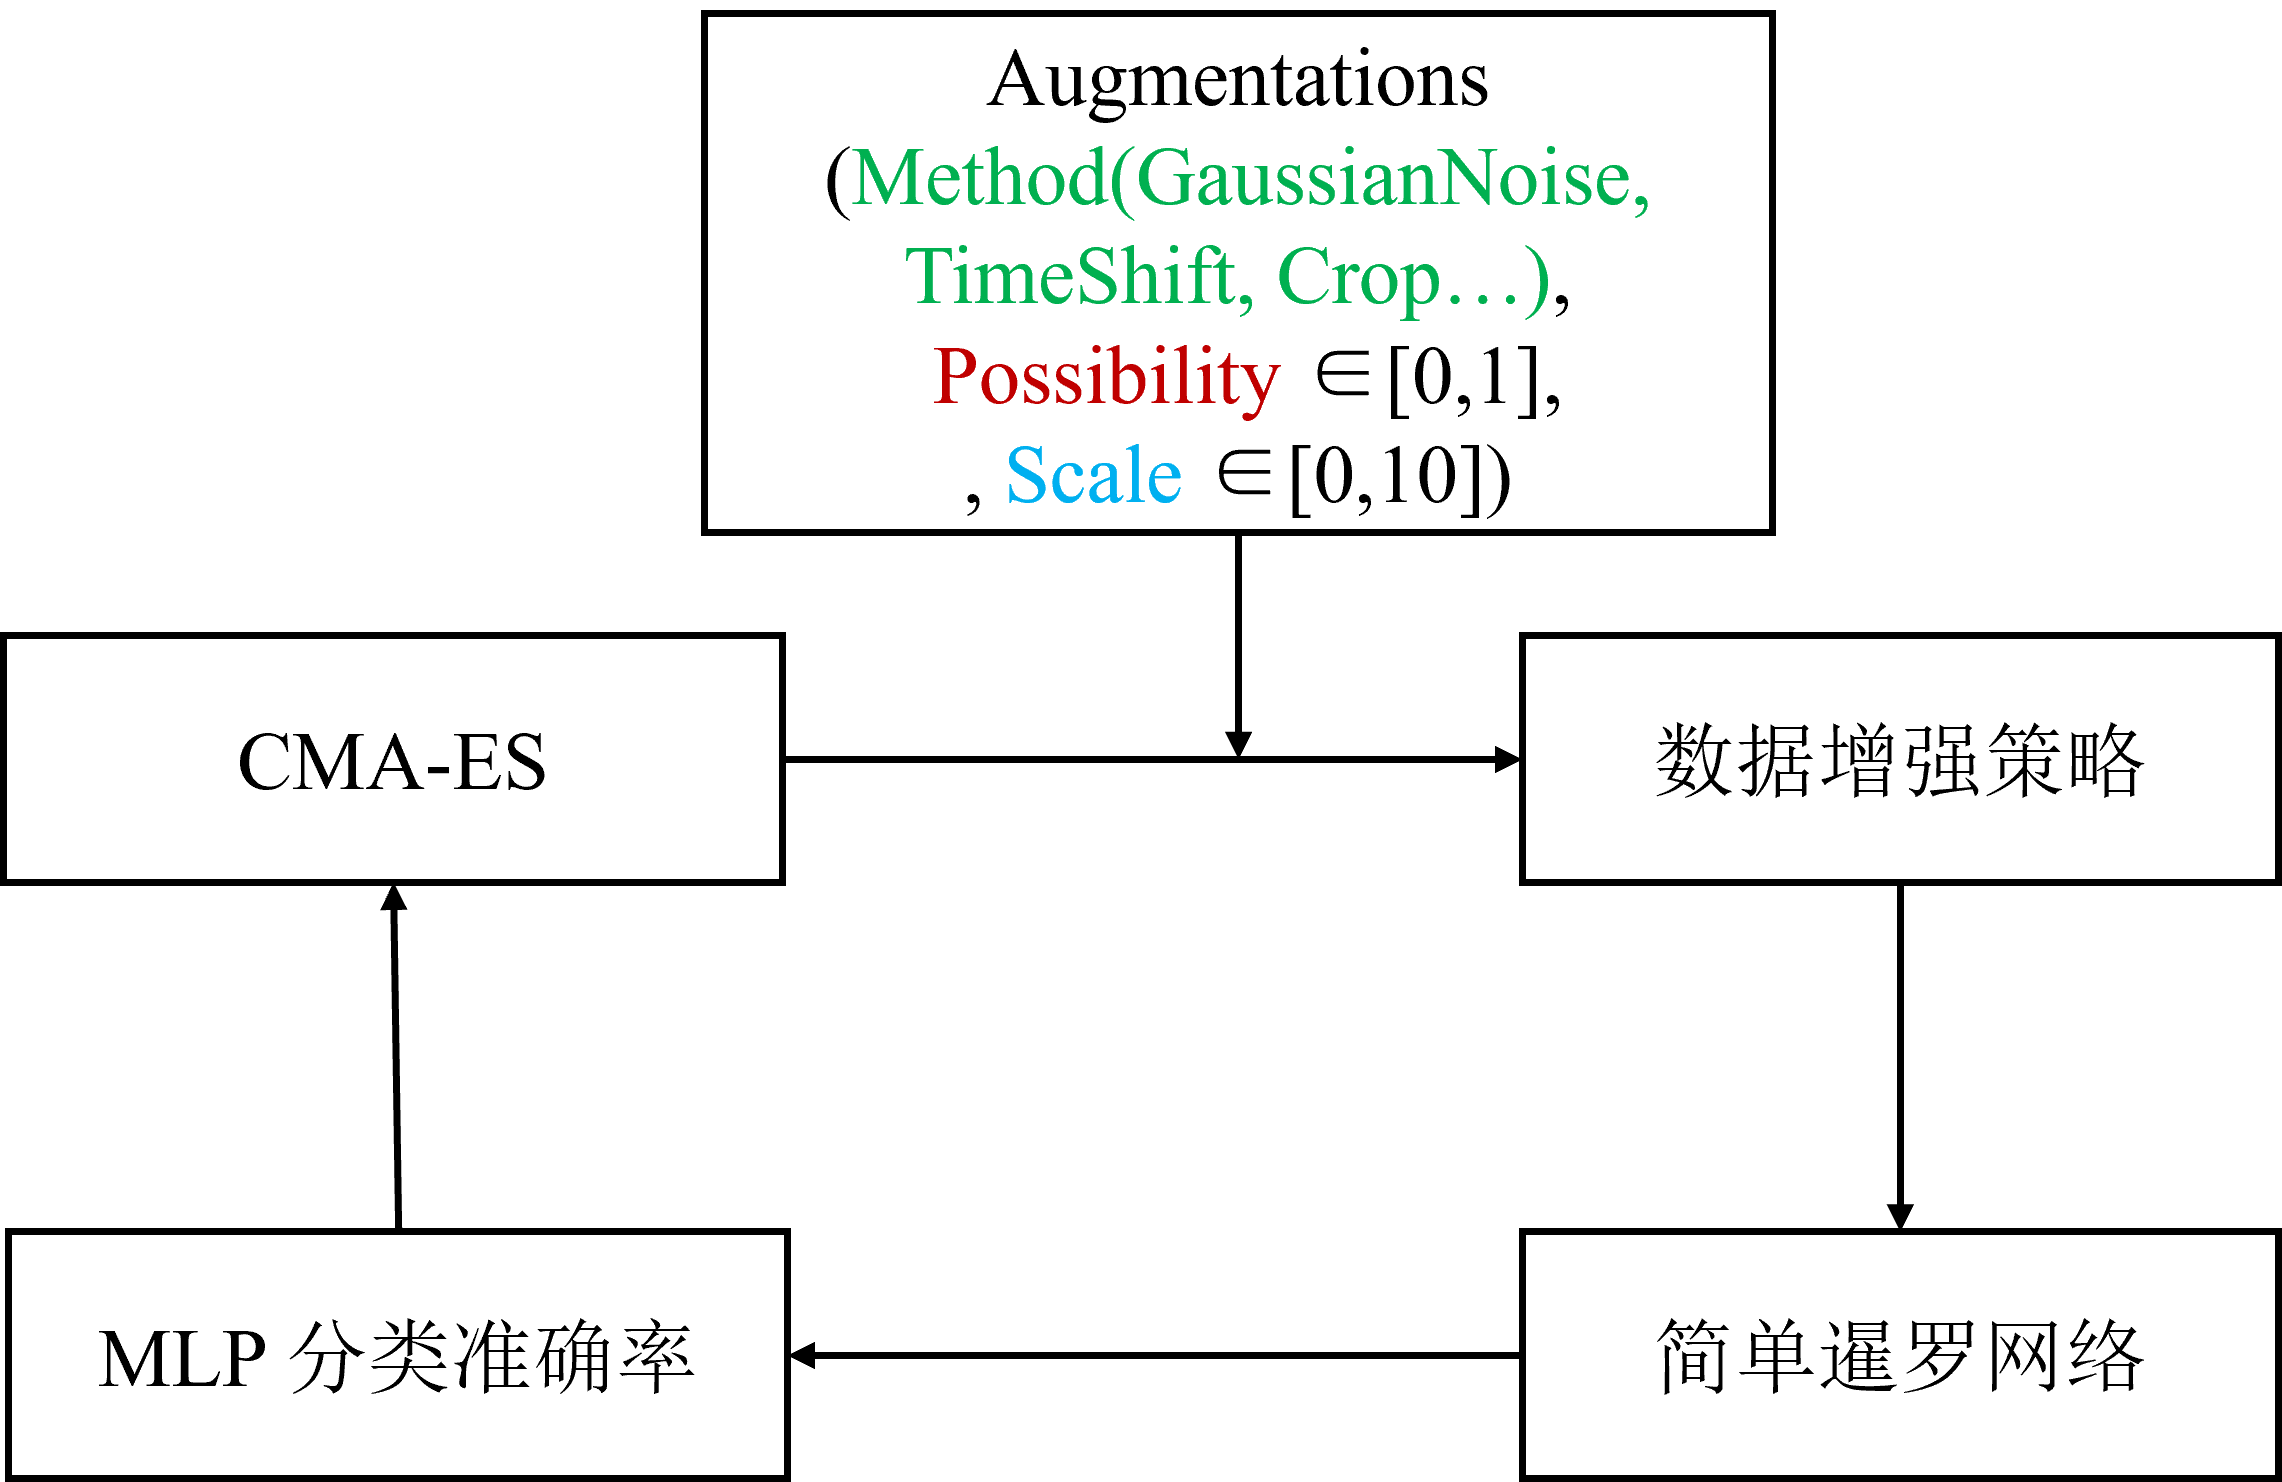
\includegraphics[width=8cm]{CMA-ES.png}
    \caption{使用CMA-ES搜索最优的数据增强策略框架概览}
    \label{CMA-ES}
\end{figure}
搜索空间细节:在我们的搜索空间中,一个策略由 9 个信号数据增强子策略组成,如图\ref{data_augmentation}所示。此外,每个操作还关联两个超参数:
\begin{itemize}
    \item 1) 应用操作的概率\(\in [0,1]\),
    \item 2) 操作的幅度映射后\(\in [0,10]\)。
\end{itemize}
以下介绍各个数据增强子策略幅度的映射:
\begin{itemize}
    \item \textbf{掩码(Random Masked)}:随机选取100个不重叠的大小为$s$的子区间,将其置0。$s$作为增强幅度由\([1,5]\)映射为\([0,10]\)。

    \item \textbf{添加高斯噪声(Adding Gaussian Noise)}:将高斯噪声的信噪比SNR作为增强幅度,由\([2,6]\)映射为\([0,10]\)。

    \item \textbf{相位扰动(Phase Perturbation)}:相位扰动服从均匀分布$\text{U}(-perturb_{\text{max}}, perturb_{\text{max}})$,$perturb_{\text{max}}$作为增强幅度由\([0.1,0.5]\)映射为\([0,10]\)。

    \item \textbf{块打乱(RandomChunkShuffle)}:将时间序列数据分割成大小均匀的$s$个块,然后随机打乱这些块的顺序。$s$作为增强幅度由\([10,100]\)映射为\([0,10]\)。

    \item \textbf{随机缩放(Random Scaled)}:缩放的幅度服从均匀分布$\text{U}(1.0-scale, 1.0+scale)$。$scale$作为增强幅度由\([0.05,0.6]\)映射为\([0,10]\)。

    \item \textbf{随机绝对值(Random Abs)}:无幅度值。

    \item \textbf{竖直翻转(Random Vertical Flip)}:无幅度值。

    \item \textbf{水平翻转(Random Horizontal Flip)}:无幅度值。

    \item \textbf{时移(Time Shift)}:无幅度值,平移的距离固定服从均匀分布$\text{U}(-512, 512)$。
\end{itemize}
则CMA-ES优化器求解的问题可以描述为 
\begin{equation}
    \arg\max_{\mathbf{p}, \mathbf{s}} \text{Accuracy}(\mathbf{p}, \mathbf{s}, \text{SimSiam-Net})
\end{equation}
其中,\(\mathbf{p}\) 和 \(\mathbf{s}\) 为求解的参数,分别满足 \(p_i \in [0, 1]\) 和 \(s_i \in [0, 10]\),Accuracy为简单暹罗网络验证的准确率。

\section{实验与分析}
\subsection{基于CMA-ES优化器的最优数据增强策略搜索}
数据集:用于SimSiam对比学习预训练的无标签数据个数为500个,用于微调的有标签数据为100个,每类各10个。CMA-ES超参数设置:变量维度为14(\(len(\mathbf{p}\))+\(len(\mathbf{s}\))),种群规模为11,迭代次数为10次。求得最优的数据增强策略如表\ref{}
\begin{table}[h]
    \caption{增强方法及其参数}
    \begin{tabular}{cccc}
    \toprule
    增强名称 & 概率$p$ & 幅度$s$ & 映射后幅度$s$\\
    \midrule
    高斯噪声 & 0.9761 & 5 \\
    相位扰动 & 0.5 & 6 \\
    \bottomrule
    \end{tabular}
    \label{tableb}
    \end{table}
\section{本章小结}


\chapter{基于K-means聚类的自监督预训练方法研究}
\section{Kmeans介绍}
\section{模型架构}
\section{实验与分析}

\chapter{其他长尾学习方法分析(CB LOSS等)}

\begin{table}[h]
\caption{计算$2m\times 2m$理想导体平板时域感应电流采用的三种存储方式的存储量比较。}
\begin{tabular}{cccc}
\toprule
\multirow{2}{*}{时间步长} & \multicolumn{3}{c}{存储方式} \\
\cmidrule{2-4}
& 非压缩存储方式 & 完全压缩存储方式 & 基权函数压缩存储方式 \\
\midrule
0.4ns & 5.59 MB & 6.78 MB & 6.78 MB\\
0.5ns & 10.17 MB & 5.58 MB & 5.58 MB \\
0.6ns & 8.38MB & 4.98 MB & 4.98 MB \\
\bottomrule
\end{tabular}
\label{tablea}
\end{table}

如图\ref{picd}所示给出了时间步长选取为0.5ns 时采用三种不同存储方式计算的平板中心处$x$方向的感应电流值与IDFT 方法计算结果的比较,……。如图\ref{pice}所示给出了存储方式为基权函数压缩存储方式,时间步长分别取0.4ns、0.5ns、0.6ns时平板中心处$x$方向的感应电流计算结果,从图中可以看出不同时间步长的计算结果基本相同。

\begin{figure}[h]
\subfloat[]{
    \label{picd}
    \includegraphics[width=6.77cm]{picd.pdf}
}
\subfloat[]{
    \label{pice}
    \includegraphics[width=7.04cm]{pice.pdf}
}
\caption{$2m\times 2m$的理想导体平板中心处感应电流$x$分量随时间的变化关系。(a)不同存储方式的计算结果与IDFT方法的结果比较;(b)不同时间步长的计算结果比较比较比较}
\label{fig2}
\end{figure}

由于时域混合场积分方程是时域电场积分方程与时域磁场积分方程的线性组合,因此时域混合场积分方程时间步进算法的阻抗矩阵特征与时域电场积分方程时间步进算法的阻抗矩阵特征相同。

\section{时域积分方程时间步进算法矩阵方程的求解}
\begin{theorem}
如果时域混合场积分方程是时域电场积分方程与时域磁场积分方程的线性组合。
\end{theorem}
\begin{proof}
由于时域混合场积分方程是时域电场积分方程与时域磁场积分方程的线性组合,因此时域混合场积分方程时间步进算法的阻抗矩阵特征与时域电场积分方程时间步进算法的阻抗矩阵特征相同。
\end{proof}
\begin{corollary}
时域积分方程方法的研究近几年发展迅速,在本文研究工作的基础上,仍有以下方向值得进一步研究。
\end{corollary}
\begin{lemma}
因此时域混合场积分方程时间步进算法的阻抗矩阵特征与时域电场积分方程时间步进算法的阻抗矩阵特征相同。
\end{lemma}

\section{本章小结}
本章首先研究了时域积分方程时间步进算法的阻抗元素精确计算技术,分别采用DUFFY 变换法与卷积积分精度计算法计算时域阻抗元素,通过算例验证了计算方法的高精度。

\chapter{全文总结与展望}

\section{全文总结}
本文以时域积分方程方法为研究背景,主要对求解时域积分方程的时间步进算法以及两层平面波快速算法进行了研究。

\section{后续工作展望}
时域积分方程方法的研究近几年发展迅速,在本文研究工作的基础上,仍有以下方向值得进一步研究:

\thesisacknowledgement
在攻读博士学位期间,首先衷心感谢我的导师XXX教授

\thesisappendix

\chapter{中心极限定理的证明}

\section{高斯分布和伯努利实验}


% Uncomment to list all the entries of the database.
% \nocite{*}

\thesisbibliography{reference}

%
% Uncomment following codes to load bibliography database with native
% \bibliography command.
%
% \nocite{*}
% \bibliographystyle{thesis-uestc}
% \bibliography{reference}
%

\thesisaccomplish{publications}

\end{document}
